%%---------------------------------------
%% Begin Revtex4 Lab Writeup
%%---------------------------------------
\documentclass[
    10pt,aps,prl,
    amsfonts,
    amssymb,
    amsmath,
    %byrevtex,
    %% draw prevents images from being included
    %% this speeds up compilation, uncomment for finished product
    draft,
    %eqsecnum,
    %galley,
    %groupedaddress,
    %preprint,
    %preprintnumbers,
    runinaddress,
    secnum,
    %secnumarabic,
    showkeys,
    %showpacs,
    superscriptaddress,
    twocolumn,
    %tightenlines,
    %unsortedaddress,
]{revtex4}

%%---------------------------------------
%% Begin Package Definitions
%%---------------------------------------
\usepackage{color}
\usepackage{graphicx}
\usepackage{verbatim}

%% graphs are made internally
\usepackage{tikz,pgfplots}
    \pgfplotsset{compat=1.12}
\usepgfplotslibrary{groupplots}
\usetikzlibrary{calc}

%% Awesome packages
\usepackage[inline]{enumitem}
\usepackage{hyperref}
%% for source code
%\usepackage{listings}
\usepackage{microtype}
\usepackage{subcaption}
    \captionsetup{compatibility=false}
\usepackage{siunitx}

%% Bibliography
\bibliographystyle{apsrev}

%%---------------------------------------
%% Begin Document
%%---------------------------------------
\begin{document}

\startpage{4}
\endpage{8}

\title{Physics Laboratory Report Template}

\author{Jeffrey P. \surname{Hafner}}
\email{jphafner@buffalo.edu}
\affiliation{Your School, NY 13486}

%% Collaborative Author
\collaboration{Lab Partner 1; Lab Partner 2; and Lab Partner 3}
\affiliation{Your School, NY 13486}

\date{\today}

%\include{revtex4_pacs}
\keywords{Physics, Laboratory, Template}

\begin{abstract}
    This document is to illustrate visually the formatting standards that
        are to be followed.
    An abstract is a one paragraph summary of your lab.
    %Your abstract should include one sentence dedicated to
    %    Introduction, Methods, Results, Conclusion.
    You should include at least one sentence dedicated to explaining
        the purpose of the lab, a simple overview of the procedure,
        a brief overview of the results, and a brief overview of
        its interpretation.
    A good rule of thumb is to construct a paragraph using one 
        sentence summaries of each section of your lab report.
    Some journals now subsection the abstract based on how the paper is divided.
\end{abstract}

\maketitle
%% NOTE: Optionally add a table of contents section
%\tableofcontents

%%---------------------------------------
%% Begin Content
%%---------------------------------------

\section{Introduction}
    \label{sec:intro}

    %% NOTE: use \ref{sec:intro} to refer to this section in text
    This is section \ref{sec:intro},
        it comes after the abstract and before section \ref{sec:methods}.

    Describe what concept/s the lab explores, 
        the main objective of the lab, 
        what actions you performed, 
        and how those actions helped you achieve the lab objective.
    Also, describe your hypothesis and how you arrived 
        at it using the scientific concepts described.

    Please notice that this template lab report fully complies
        with the American Physical Society's Style and Notation
        Guidelines for their publications.

    While your lab report is not required to be formatted for publication,
        it should strive to achieve it.
    By abiding by professional standards, you too can help ensure
        that your lab report is as clear and concise as possible.
   
    For more information, please refer to the American Physical's
        Society's Guide for its publications
    %% NOTE: use \footnote{ } to include footnotes,
    %% NOTE: use \cite{ } to include citations, 
    %% NOTE: citation infomation must be in revtex4_example.bib
    \footnote{\url{http://forms.aps.org/author/styleguide.pdf}}
    \footnote{\url{http://journals.aps.org/revtex/}}
    \footnote{\url{http://journals.aps.org/author-information}}
    \cite{Simon:2010:SIGCSE}
    \cite{PeerInstruction}.

    For information concerning how to write,
        Refer to the Mayfield Manual\cite{Mayfield},
        or the Elements of Style\cite{StrunkWilliam}.

    For unit style conventions, refer to the ``Checklist for Reviewing Manuscripts''
        in The NIST Guide for the use of the International System of Units\cite{NISTsp811}.

    %% NOTE: the [h,b,t] to place the figure preferentially on page
    %% NOTE: h: here, b: bottom of page, t: top of page
    \begin{table}[h]
        \begin{ruledtabular}
        %% this is a 5 column table with centered elements
        \begin{tabular}{c|ccc|c}
            %% The ampersand is used to denote the start of a new column
            $l/(\si{\meter})$ &
            $t_1/(\si{\second})$ &
            $t_2/(\si{\second})$ &
            $t_3/(\si{\second})$ &
            %% The \\ is used to denote the start of a new row
            $t_{ave}/(\si{\second})$ \\
            %% \hline makes a nice horizontal rule for organization
            \hline
            0.2 &  8.9 &  8.6 &  8.9 &  8.8 \\
            0.4 & 12.8 & 12.6 & 12.9 & 12.8 \\
            0.6 & 15.8 & 15.6 & 15.0 & 15.5 \\
            0.8 & 18.0 & 18.1 & 17.5 & 17.9 \\
            1.0 & 20.0 & 20.2 & 20.0 & 20.1 \\
        \end{tabular}
        \end{ruledtabular}
        %% You should always use a caption
        \caption{An example caption for experimentally observed data.}
        %% NOTE: use \ref{tab:data} to refer to table in text
        \label{tab:data}
    \end{table}

    \begin{figure}
        \centering
        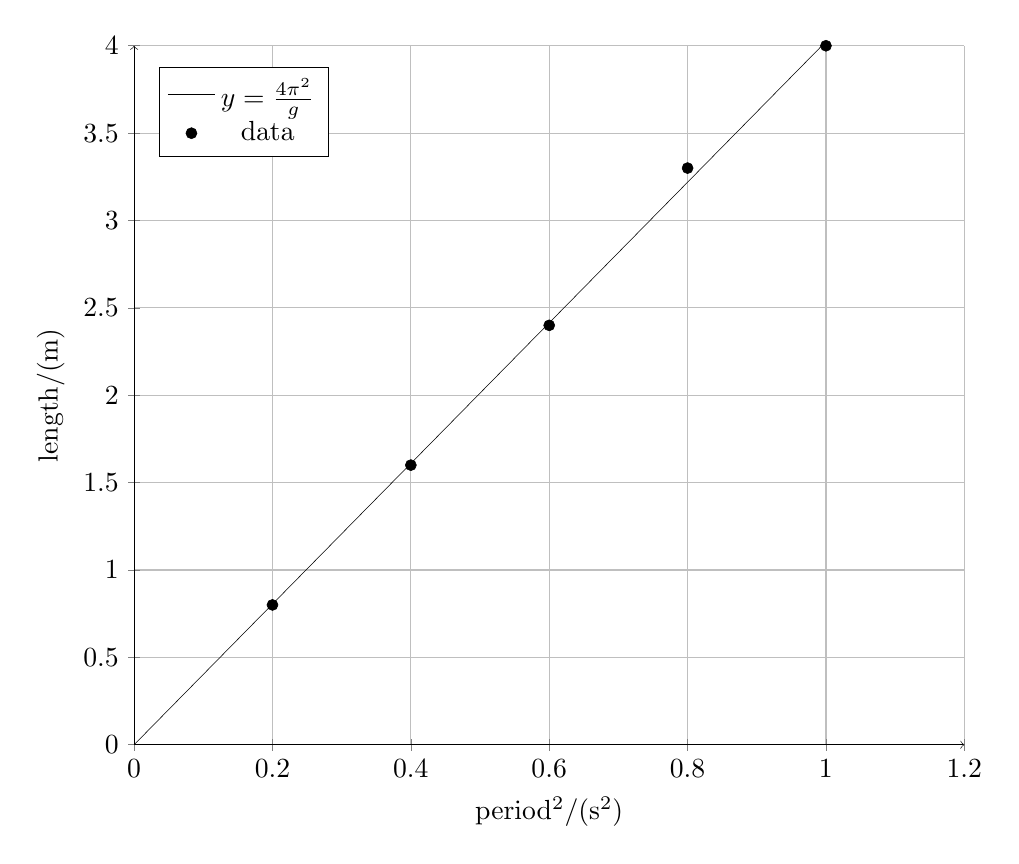
\begin{tikzpicture}[x=0.4\linewidth]
            \begin{axis}[
                %%% Plot defintiions go here
                axis y line=left,
                axis x line=bottom,
                axis line style={->},
                xlabel=period\textsuperscript{2}/(\si{\second\squared}),
                ylabel=length/(\si{\meter}),
                xmin=0,
                xmax=1.2,
                ymin=0,
                %height=9cm,
                width=\linewidth,
                grid=major,
                very thin,
                legend style={at={(0.03,0.97)}, anchor=north west}
            ]
            %% enter best fit line here
            \addplot[no marks]{4.024 * x};
            %% best fit line label here
            \addlegendentry{$y=\frac{4\pi{}^2}{g}$}
            %% Enter data points here for graph
            \addplot[only marks] coordinates {
                %% X,Y
                (0.2,0.8)
                (0.4,1.6)
                (0.6,2.4)
                (0.8,3.3)
                (1.0,4.0)
            };
            \addlegendentry{data}
            \end{axis}
        \end{tikzpicture}
        \label{fig:data-plot}
        \caption{Plot of the Period of one oscillation squared verses length of pendulum}
    \end{figure}

    %% NOTE: you can optionally make the graph externally and import with graphicx
    \begin{figure}
        %% NOTE: alternativily you can specifc width=, or height=
        
\includegraphics[width=\linewidth,keepaspectratio]{placeholder}
        \label{fig:alt-data}
        \caption{example of importing an external filename}
    \end{figure}


%% Begin Methods
%%---------------------------------------
\section{Methods}
    \label{sec:methods}

    Document your experimental procedure in enough detail that someone
        else could repeat your work. 
    This should include a list of all materials used, a diagram of the
        lab setup if appropriate, and the steps taken to accomplish the
        lab (paragraphs preferred, but organized, ordered lists of
        instructions are acceptable with list items in complete sentences.)

    %% NOTE: an example of a list
    %% NOTE: use \begin{enumerate} if you want the list numbered
    \begin{itemize}
        \item Materials: List all materials used.
        \item Diagrams: Show schematic of experimental setup where necessary.
        \item Steps Taken: Provide enough information that another student
                could easily replicate your work.
    \end{itemize}

    %\begin{figure}
    %\begin{tikzpicture}
    %\end{tikzpicture}
    %\end{figure}

%% Begin Results
%%---------------------------------------
\section{Results}
    \label{sec:results}

    Put your data into tables and graphs. 
    Review your tables and graphs to determine the key findings from the
        lab exercise. 
    Write a paragraph explaining each table and graph including its key
        result and other salient details.
    Arrange the results section in an organized fashion.
    \begin{itemize}
        %% NOTE: inline lists, using itemize*, are much preferred, LEAST INK!!
        \item Data Tables: Organized and labeled with units.
        \item Graphs: Properly label all axes, provide appropriate title.
        \item Explanations: The key relationship from each table or graph
                 is described in a separate paragraph with appropriate 
                 supporting details.
    \end{itemize}

    %% NOTE: use \begin{table*} for fullwidth table
    \begin{table*}
        \begin{ruledtabular}
        \begin{tabular}{ccc}
                          & first       & second  \\
            independent   & dependent   & dependent \\
             variable     & variable    & variable \\
            \hline
            X1 & Y1 & Z1 \\
            X2 & Y2 & Z2 \\
            X3 & Y3 & Z3 \\
            X4 & Y4 & Z4 \\
            X5 & Y5 & Z5 \\
            X6 & Y6 & Z6 \\
        \end{tabular}
        \end{ruledtabular}
        \label{tab:data-table}
        \caption{Caption for experimental data table,
            please note that it is not necessary placed inline to where it is in the source file}
    \end{table*}

    %% NOTE: use \begin{figure*} for fullpage figure
    \begin{figure*}
    \begin{tikzpicture}
        \begin{axis}[
            %width=190pt,
            width=\linewidth,
            axis x line=middle,
            axis y line=center,
            tick align=outside]
        \addplot+[mark=none,smooth] (\x,\x);
        \end{axis}
    \end{tikzpicture}
    \label{fig:data-graph}
    \caption{Caption for experimental data graph,
        please note that it is not necessarily placed inline to where it is in the source file}
    \end{figure*}

%% Begin Discussion
%%---------------------------------------
\section{Discussion}
    \label{sec:discussion}

    Explain whether results support the hypothesis, 
        with supporting details referenced from the results section. 
    Explain why results support or do not support the hypothesis. 
    Discuss any problems encountered, 
        uncertainty in measurements, 
        comparison to others performing the lab, 
        and possible improvement opportunities

%% Begin Conclusion
%%---------------------------------------
\section{Conclusion}
    \label{sec:conclusion}
    What did you learn from this lab about the concept under study? 
    Include appropriate supporting details. 
    Did you learn anything else from the lab, 
        such as use of lab equipment, procedures,
        analysis methods, etc\dots{}?


%% Begin Appendix
%%---------------------------------------
\appendix

\section{Rubric}
\label{sec:rubric}
    The lab report will be graded based on four different elements.
    Argument, Technical Style, Use of Physics, and Quantitativeness.
    With many thanks to the University of Minnesota Physics Department\cite{UMNrubric}.

    \textbf{Argument:}
    \begin{itemize*}
        \item complete, cogent, flowing argument
        \item context, execution, analysis, conclusion all present
        \item leaves reader satisfied
    \end{itemize*}

    \textbf{Technical Style:}
    \begin{itemize*}
        \item language is appropriate
        \item nonverbal media present where appropriate, well constructed, well incorporated
        \item objective, indicative, logical style
        \item consistent style
        \item division into sections is helpful
    \end{itemize*}

    \textbf{Use of Physics:}
    \begin{itemize*}
        \item predictions are justified with physical theory
        \item experiment is physically sound and actually tests phenomenon in question
        \item results interpreted with theory to clear, appropriate conclusion
    \end{itemize*}

    \textbf{Quantitativeness:}
    \begin{itemize*}
        \item consistently quantitative
        \item equations, numbers with units, uncertainties throughout
        \item prediction confirmed or denied, result found by error analysis
        \item results, conclusions based on data
    \end{itemize*}

\section{Checklist}
    As any physics teacher will tell you,
        units are the single most common mistake that physics students will make.
    It is highly recommended that you review the NIST Checklist for Reviewing Manuscripts\cite{NISTsp811}.
    I am listing this checklist twice,
        because it is \emph{twice} as important as everything else.

    Before submitting your report, please verify that all necessary elements are present.
    While this list will not be used for grading,
        it is a good idea to use it to double check your report.
    With many thanks to Chad Orzel\cite{Orzel}.

    \textbf{Abstract:}
    \begin{itemize*}[label=\square]
        \item Summarize in paragraph form
        \item State results
        \item Uncertainty and units
    \end{itemize*}

    \textbf{Introduction:}
    \begin{itemize*}[label=\square]
        \item Discuss motivation of experiment
        \item Describe theory being tested
        \item Describe specific prediction of interest
    \end{itemize*}

    \textbf{Experimental Procedure:}
    \begin{itemize*}[label=\square]
        \item Write out in paragraph form
        \item Describe apparatus used
        \item Include only important details
        \item Explain measurements made
        \item Include uncertainty estimates
    \end{itemize*}

    \textbf{Results:}
    \begin{itemize*}[label=\square]
        \item Write out in paragraph form
        \item Clearly labeled data tables
        \item Units, uncertainties
        \item Figures (where appropriate)
        \item Labels on figures
        \item Refer to figures and tables in text
        \item Calculations from data
        \item Errors and uncertainties in calculations
    \end{itemize*}

    \textbf{Discussion/Conclusion:}
    \begin{itemize*}[label=\square]
        \item Summarize results of experiment
        \item Further interpretations, implications
        \item Agreement/ disagreement with predictions
        \item Comparison of methods (where appropriate)
        \item Possible improvements
    \end{itemize*}

    \textbf{General Writing:}
    \begin{itemize*}[label=\square]
        \item Organization
        \item Sentence structure, grammar
        \item Spelling, proofreading
    \end{itemize*}


%% Begin Equations Appendix
%%---------------------------------------

\section{Equations}
This is just a section filled with random items as reference.

The Maxwell equations of Electromagnetism with equation alignment using align and the ampersand,
    which is a ligature of et, which means and in Latin:
\begin{align}
    \del\cdot\mathbf{E} &= \dfrac{\rho}{\epsilon_0} \\
    \del\cdot\mathbf{B} &= 0 \\
    \del\times\mathbf{E} &= \dfrac{\partial\mathbf{B}}{\partial t} \\
    \del\times\mathbf{B} &= \mu_0 \left(\mathbf{J} + \epsilon_0 \dfrac{\partial\mathbf{E}}{\partial t} \\
\end{align}

%% NOTE: that units are typed in roman fonts, not italic fonts as variables are!!
%% NOTE: also note that there is a forced small space between the number and units!!
Some inline scientific notation $4.0\times 10^{-3}\,\mathrm{N/m}$\cite{NISTsp811},
    and some more that is in displaystyle
\begin{equation}
    4.0\times 10^{-3}\,\mathrm{N/m}
\end{equation}
Some simple equation
\begin{equation}
    \Delta =\sum_{i=1}^N w_i (x_i - \bar{x})^2.
\end{equation}
\begin{equation}
    %% NOTE: use nonumber to remove the equation numbering,
    %%      or equation* instead of equation
    %% NOTE: YOU SHOULD NEVER REMOVE THE EQUATION NUMBERING!!
    P(x) = \frac{x - a}{b - a}, \nonumber
\end{equation}
\begin{equation}
    g = \frac{1}{2} \sqrt{2\pi}. \nonumber
\end{equation}

More complex equations, equation \ref{eq:ising} is below.
\begin{equation}
    %% NOTE: you can reference this with \ref{eq:ising} in the text
    \label{eq:ising}
    E = -J \sum_{i=1}^N s_i s_{i+1},
\end{equation}
\begin{equation}
    I = \! \int_{-\infty}^\infty f(x)\,\mathrm{d}x \label{eq:fine}.
\end{equation}

Align multiple equations
\begin{align}
    a & = b \\
    c &= d,
\end{align}

We can also have different cases:
\begin{equation}
\label{eq:mdiv}
m(T) =
\begin{cases}
0 & \text{($T > T_c$)} \\
\big(1 - [\sinh 2 \beta J]^{-4} \big)^{\! 1/8} & \text{($T < T_c$)},
\end{cases}
\end{equation}

write matrices
\begin{align}
\textbf{T} &=
\begin{pmatrix}
T_{++} \hfill & T_{+-} \\
T_{-+} & T_{--} \hfill 
\end{pmatrix}, \nonumber \\
& =
\begin{pmatrix}
e^{\beta (J + B)} \hfill & e^{-\beta J} \hfill \\
e^{-\beta J} \hfill & e^{\beta (J - B)} \hfill
\end{pmatrix}.
\end{align}

\section{Common Greek letters}

These commands may be used only in math mode. 
%% Math mode is surounded by cash symbols
%%  or math environment brackets, equation, align, etc...
Only the most common letters are included here.
$\alpha$, $\beta$, $\gamma$, $\Gamma$, $\delta$, $\Delta$, $\epsilon$, $\zeta$, $\eta$, $\theta$, $\Theta$, $\kappa$, $\lambda$, $\Lambda$, $\mu$, $\nu$, $\xi$, $\Xi$, $\pi$, $\Pi$, $\rho$, $\sigma$, $\tau$, $\phi$, $\Phi$, $\chi$, $\psi$, $\Psi$, $\omega$, $\Omega$



%% Begin Acknowledgments
%%---------------------------------------
\section{Acknowledgments}
\label{sec:ack}
\begin{acknowledgments}
    %% NOTE: if you received any financial support, this is required for tracking purposes
    Resources for this laboratory were provided by ``a school''.
    Special thanks and acknowledgments for the guidance provided by Dr. Jeffrey P. Hafner.
\end{acknowledgments}

%% Begin Bibliography
%%---------------------------------------

%% NOTE: this is where we define our bibiliography file for references
\bibliography{revtex4_example}

%%---------------------------------------
%% End Document
%%---------------------------------------
\end{document}


